\documentclass{article}
\usepackage{ctex}
\usepackage{graphicx}
\usepackage{geometry}
\geometry{left=2.5cm,right=2.5cm,top=2.5cm,bottom=2.5cm}
\usepackage{float}
\usepackage{hyperref}
\hypersetup{hidelinks}
\usepackage{enumitem}
\usepackage{listings}
\usepackage{xcolor}
\usepackage{titlesec}
\usepackage{fancyhdr}
\usepackage{amsmath}
\usepackage{caption}
\usepackage{subcaption}

% === Code style ===
\lstset{
    basicstyle=\small\ttfamily,
    columns=flexible,
    extendedchars=true,
    breaklines=true,
    frame=single,
    numbers=left,
    numberstyle=\tiny,
    backgroundcolor=\color{gray!5},
    language=C++
}

% === Header ===
\pagestyle{fancy}
\fancyhf{}
\fancyhead[L]{计算机图形学课程实验报告}
\fancyhead[R]{\thepage}
\renewcommand{\headrulewidth}{0.4pt}
\setlength{\headheight}{14.5pt}

\title{\textbf{计算机图形学课程实验报告}\\[6pt]
       \large 基于OpenGL的三维图形引擎与Minecraft风格游戏}

\begin{document}

% ============================================================
% Title Page
% ============================================================
\begin{titlepage}
    \centering
    \vspace*{2cm}
    \begin{center}
        \zihao{1}\heiti
        计算机图形学课程实验报告
    \end{center}
    \newcommand\ful[2][5cm]{\underline{\makebox[#1][c]{#2}}}
    \vskip 1.5cm
    \begin{center}
        \zihao{2}\heiti
        基于OpenGL的三维图形引擎\\[4pt]
        与Minecraft风格游戏
    \end{center}
    \vskip 2.5cm
    \begin{center}
        \zihao{4}
        姓\hspace{1em}名：\ful{杨征雨}\\[12pt]
        学\hspace{1em}号：\ful{3230105712}\\[12pt]
        学\hspace{1em}院：\ful{竺可桢学院}\\[12pt]
        专\hspace{1em}业：\ful{人工智能}
    \end{center}
    \vfill
    \Large
    \today
\end{titlepage}

\newpage
\tableofcontents
\newpage

% ============================================================
\section{项目概述}
% ============================================================

本项目实现了一个基于 OpenGL 3.3 和 C++17 的三维图形渲染引擎，并在此基础上构建了一款具有可玩性的 Minecraft 风格第一/第三人称沙盒游戏\texttt{final\_project}。

\subsection{技术栈}
\begin{itemize}[nosep]
    \item \textbf{图形API：} OpenGL 3.3 Core Profile
    \item \textbf{语言：} C++17
    \item \textbf{窗口管理：} GLFW 3.x
    \item \textbf{数学库：} GLM (OpenGL Mathematics)
    \item \textbf{GUI：} Dear ImGui
    \item \textbf{图像加载：} stb\_image
    \item \textbf{构建系统：} CMake 3.15+
\end{itemize}

\subsection{工程结构}
项目采用模块化设计，核心代码位于\texttt{src/}目录下：
\begin{itemize}[nosep]
    \item \texttt{src/base/} —— 基础组件（应用框架、相机、纹理、FBO、天空盒等）
    \item \texttt{src/mesh/} —— 网格数据结构
    \item \texttt{src/primitives/} —— 基本体素生成（立方体、球、圆柱等）
    \item \texttt{src/obj\_loader/} —— OBJ 文件导入导出
    \item \texttt{src/render\_util/} —— Phong 光照着色器封装
    \item \texttt{src/collision/} —— AABB 碰撞检测
    \item \texttt{src/animation/} —— 骨骼动画系统
    \item \texttt{src/nurbs/} —— NURBS 曲面建模
    \item \texttt{src/camera/} —— 自由相机
    \item \texttt{src/orbit\_control/} —— 轨道控制器
    \item \texttt{src/game/} —— 游戏逻辑（世界生成、碰撞、敌人、箭塔等）
\end{itemize}

% ============================================================
\section{基本功能实现}
% ============================================================

\subsection{基本体素建模}

引擎支持以下基本图元的程序化生成（\texttt{src/primitives/primitives.cpp}）：

\begin{itemize}[nosep]
    \item \textbf{立方体 (Cube)} —— 带法线的 36 顶点立方体，支持任意尺寸缩放
    \item \textbf{球体 (Sphere)} —— 基于经纬度细分的三角网格
    \item \textbf{圆柱体 (Cylinder)} —— 可指定上下半径和段数
    \item \textbf{圆锥体 (Cone)} —— 圆柱体的退化情况（一端半径为 0）
    \item \textbf{多面棱柱 / 棱台} —— 通过正多边形底面扫掠实现
\end{itemize}

游戏场景中大量使用立方体实例化渲染（instanced rendering），单次 draw call 即可绘制同一类型的所有方块。门框由 4 个缩放立方体（左右柱 + 上下梁）拼接而成。

\subsection{三维网格导入导出 (OBJ)}

\texttt{src/obj\_loader/obj\_loader.cpp} 实现了完整的 Wavefront OBJ 格式读写：

\begin{itemize}[nosep]
    \item \textbf{导入：} 解析 \texttt{v}, \texttt{vt}, \texttt{vn}, \texttt{f} 行，支持三角面和四边面
    \item \textbf{导出：} \texttt{Save()} 函数将内存中的 Element 结构序列化为标准 OBJ 文件
    \item \textbf{UI 集成：} 游戏内可从 \texttt{media/obj/} 目录浏览和选择 OBJ 模型放置在场景中
    \item \textbf{场景导出：} 可将当前所有方块体素一键导出为 \texttt{exported\_scene.obj}
\end{itemize}

\subsection{材质与纹理}

引擎支持两种着色器模式：

\begin{itemize}[nosep]
    \item \textbf{纯色模式}（\texttt{SimpleLitShader}）：每种方块类型有独立的 Phong 材质颜色
    \item \textbf{纹理模式}（\texttt{TexturedLitShader}）：使用程序化生成的纹理图集（atlas）
\end{itemize}

\subsubsection{纹理图集}
系统在运行时生成 $1024 \times 1024$ 像素的纹理图集（\texttt{buildTextureAtlas()}），分为 8 列（每 tile $128 \times 128$），包含：
\begin{itemize}[nosep]
    \item 草方块（顶面绿 + 侧面土 + 底面土，共 3 tile）
    \item 泥土、石头、木头、树叶、沙子 —— 各占 1 tile
    \item 水面 —— 带半透明的蓝色 tile
    \item 总计 9 种方块类型的完整纹理
\end{itemize}

Fragment Shader 中根据顶点法线方向动态选择对应的 tile（顶面 / 底面 / 侧面），实现类似原版 Minecraft 的方块纹理映射。

\subsection{几何变换}

系统通过 GLM 库支持完整的仿射变换管线：
\begin{itemize}[nosep]
    \item \textbf{TRS 模型矩阵：} 每个物体的 \texttt{model = translate * rotate * scale}
    \item \textbf{用户交互：} ImGui 面板可实时编辑选中物体的平移、旋转、缩放参数
    \item \textbf{相机变换：} 透视投影（FOV 60°）+ 观察矩阵，支持第一/第三人称切换
    \item \textbf{光源变换：} 太阳方向、点光源位置均可通过 UI 实时调整
\end{itemize}

\subsection{光照模型}

基于 Blinn-Phong 模型实现，包含三层光源（完整 shader 见 \texttt{src/render\_util/simple\_lit.h}），公式如下：

\[
\begin{aligned}
L = &\underbrace{k_a \cdot C \cdot (0.5 + 0.5 N_y)}_{\text{半球环境光}} \\
    &+ \underbrace{S \cdot \big[k_d \cdot C \cdot (N \cdot L) + k_s \cdot (R \cdot V)^\alpha\big]}_{\text{平行光 diffuse+specular}} \\
    &+ \underbrace{\frac{I}{k_c + k_l d + k_q d^2} \cdot C_p \cdot \big[\text{diffuse} + \text{specular}\big]}_{\text{点光源}}
\end{aligned}
\]

其中 $S$ 为阴影因子（见第 \ref{sec:shadow} 节）。最终输出经过 Gamma 校正（$\gamma = 2.2$）。

\subsubsection{光源编辑}
通过 ImGui 面板可实时编辑：
\begin{itemize}[nosep]
    \item 太阳方向向量、颜色（暖色调 1.0/0.95/0.85）
    \item 环境光强度
    \item 点光源位置、颜色、强度
    \item 点光源衰减系数（$k_c$, $k_l$, $k_q$）
    \item 镜面高光指数、颜色
    \item 阴影开关及阴影偏移量
\end{itemize}

\subsection{场景漫游}

提供三种相机模式：

\begin{itemize}[nosep]
    \item \textbf{第三人称轨道相机（默认）：} 鼠标右键拖拽旋转（Orbit），滚轮缩放（Zoom In/Out），中键平移（Pan）。基于 Arcball 旋转实现，操作流畅
    \item \textbf{第一人称：} WASD 移动 + 鼠标控制视角，带碰撞检测，适合游戏体验。按 \texttt{F} 键切换
    \item \textbf{全局缩放 (Zoom To Fit)：} 场景加载时自动调整相机距离以适应场景包围盒
\end{itemize}


\begin{figure}[H]
    \centering
    \begin{subfigure}{0.48\textwidth}
        \centering
        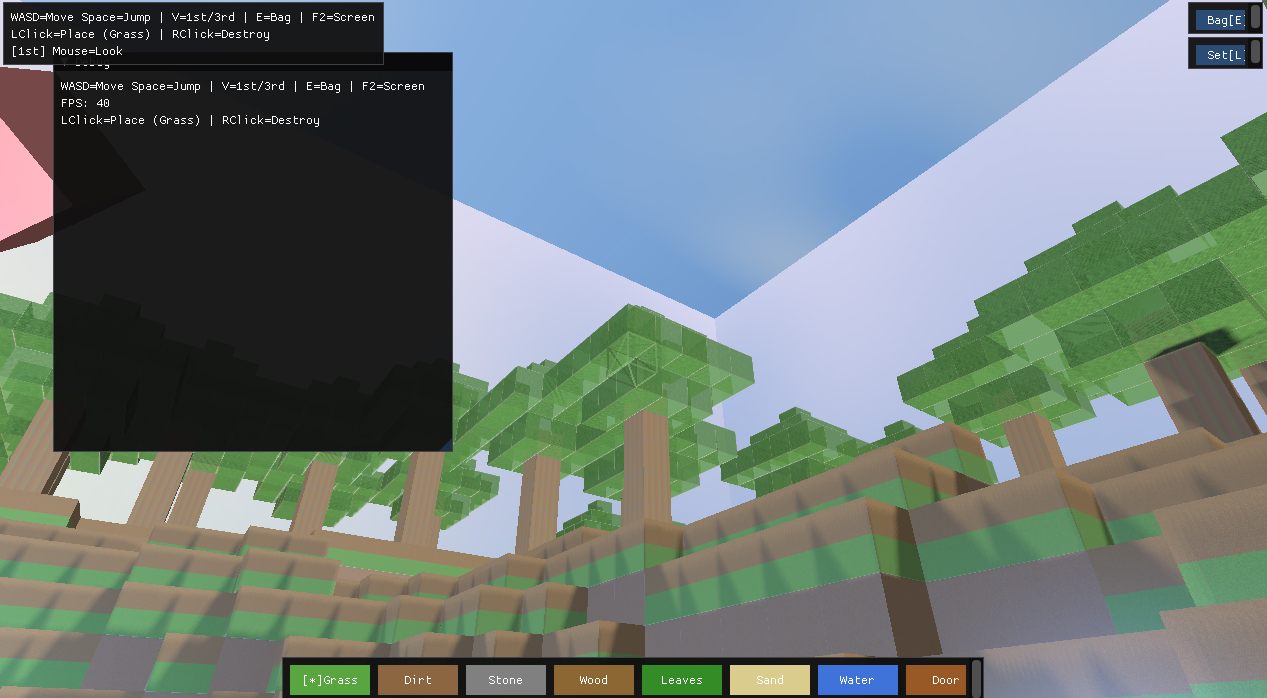
\includegraphics[width=\textwidth]{figures/1.png}
        \caption{第一人称视角}
        \label{fig:first_person}
    \end{subfigure}
    \hfill
    \begin{subfigure}{0.48\textwidth}
        \centering
        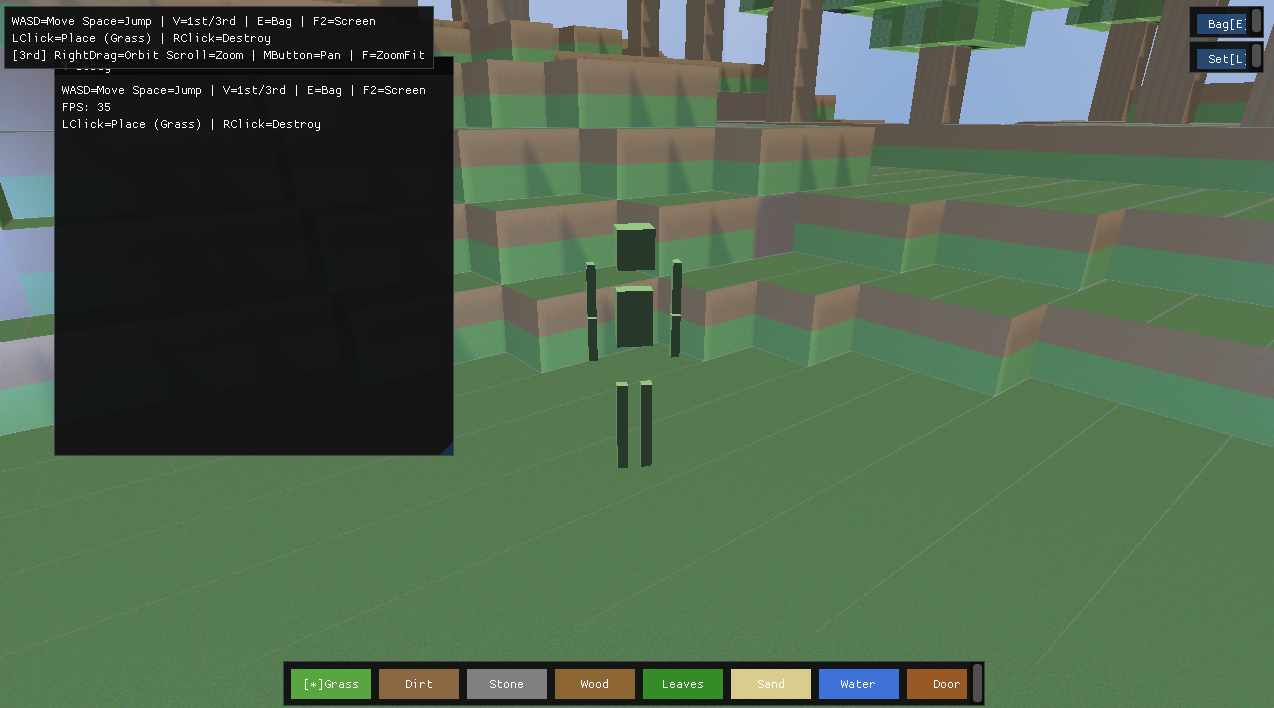
\includegraphics[width=\textwidth]{figures/3.png}
        \caption{第三人称视角}
        \label{fig:third_person}
    \end{subfigure}
    \caption{第一人称与第三人称视角对比}
    \label{fig:camera_modes}
\end{figure}



相机参数（FOV、近远裁剪面）均可在代码中调整。支持 \texttt{glm::perspective} 和 \texttt{glm::lookAt} 标准投影。

\subsection{动画播放}

引擎内置完整的骨骼动画系统（\texttt{src/animation/}）：
\begin{itemize}[nosep]
    \item \textbf{骨骼层次结构：} \texttt{Skeleton} 类维护关节树，支持递归的世界矩阵计算
    \item \textbf{蒙皮网格：} \texttt{SkinnedMesh} 支持最多 4 骨骼混合的顶点蒙皮（vertex skinning），双四元数插值
    \item \textbf{动画片段：} \texttt{AnimationClip} 导入 GLTF 动画数据，\texttt{Animator} 控制播放、混合、过渡
    \item \textbf{人形角色：} \texttt{HumanoidBuilder} 程序化生成人形骨骼 + mesh，\texttt{Humanoid} 类管理动画状态机
    \item \textbf{游戏集成：} 主角在场景中播放 idle/walk/jump 动画，状态由 \texttt{\_animState} 控制
\end{itemize}

\subsubsection{屏幕截图}
按 \texttt{P} 键可保存当前帧到 \texttt{screenshots/} 目录，使用 stb\_image\_write 输出 PNG 格式。

% ============================================================
\section{扩展功能实现}
% ============================================================

\subsection{NURBS 曲面建模}

\texttt{src/nurbs/nurbs.h} 中实现了完整的 NURBS 曲面自主算法：

\begin{itemize}[nosep]
    \item \textbf{B-spline 基函数：} 实现了 Cox-de Boor 递推公式
    \item \textbf{NURBS 曲面求值：} 双参数域采样，支持任意阶数（degree）和控制点网格
    \item \textbf{可视化：} 可切换线框/实体模式，动态调整曲面细分精度
    \item \textbf{独立演示：} \texttt{08\_nurbs} 示例程序展示 NURBS 曲面建模效果
\end{itemize}

\subsection{实时碰撞检测}
\label{sec:collision}

碰撞检测基于空间几何 AABB（Axis-Aligned Bounding Box），具有完整的实用性：

\subsubsection{核心算法（\texttt{src/collision/aabb.h}）}
\begin{itemize}[nosep]
    \item \textbf{AABB 定义：} \texttt{AABB::fromMinMax(min, max)} 构造轴对齐包围盒
    \item \textbf{重叠判断：} 六轴分离检测（SAT 在轴对齐情况下的简化）
    \item \textbf{滑动碰撞：} \texttt{collideAndSlide()} 实现经典的 AABB vs 网格滑动碰撞解析
          \begin{itemize}
              \item 先 Y 轴、再 X/Z 轴分步检测，模拟沿表面滑动的效果
              \item 玩家半宽收窄处理（margin）避免卡墙角
              \item 自动检测 \texttt{onGround} 状态用于跳跃逻辑
          \end{itemize}
\end{itemize}

\subsubsection{门碰撞系统}
专门实现了门的碰撞状态机（\texttt{resolvePlayerMovement()} 中）：

\begin{itemize}[nosep]
    \item \textbf{关闭状态：} 门区域（含门扇+门框）作为一个完整实心 AABB，不可通行
    \item \textbf{打开/动画中：}
          \begin{itemize}
              \item 门扇碰撞使用旋转后 AABB（$\cos\theta$, $\sin\theta$ 计算真实半轴），按最短重叠轴推出
              \item 左右门柱 AABB（\texttt{lb}, \texttt{rb}）始终阻挡玩家
              \item 顶部门梁 AABB（\texttt{tb}）阻止从上方穿过
              \item 底部门槛不阻挡，允许玩家自由出入
          \end{itemize}
    \item \textbf{动画过渡：} 门从 0° 平滑旋转到 90°（或反向），动画过程中碰撞 AABB 连续更新
    \item \textbf{交互：} 按 \texttt{O} 键在 3.5 范围内开关最近的门
\end{itemize}

\subsubsection{其他碰撞应用}
\begin{itemize}[nosep]
    \item 玩家移动、跳跃、重力均经过碰撞检测约束
    \item 投射物（箭矢）与方块碰撞检测
    \item 敌人寻路避开障碍物
\end{itemize}

\subsection{实时阴影映射}
\label{sec:shadow}

实现了标准的 Shadow Mapping + PCF 软阴影：

\subsubsection{Shadow Pass（\texttt{renderShadowPass()}）}
\begin{itemize}[nosep]
    \item 2048×2048 深度纹理（\texttt{GL\_DEPTH\_COMPONENT}, float）
    \item 正交投影光源空间矩阵：以玩家位置为中心，范围 30×30
    \item 使用 \texttt{glCullFace(GL\_FRONT)} 消除 peter-panning 伪影
    \item 深度着色器仅写入深度，不输出颜色
\end{itemize}

\subsubsection{PCF 软阴影（Fragment Shader 中）}
\begin{itemize}[nosep]
    \item $5 \times 5 = 25$ 次邻域采样，加权平均得到柔和阴影边缘
    \item 手动深度比较（非硬件 PCF），完整的 bias 控制
    \item 阴影仅作用于太阳平行光（点光源无阴影，避免性能问题）
\end{itemize}

\begin{figure}[H]
    \centering
    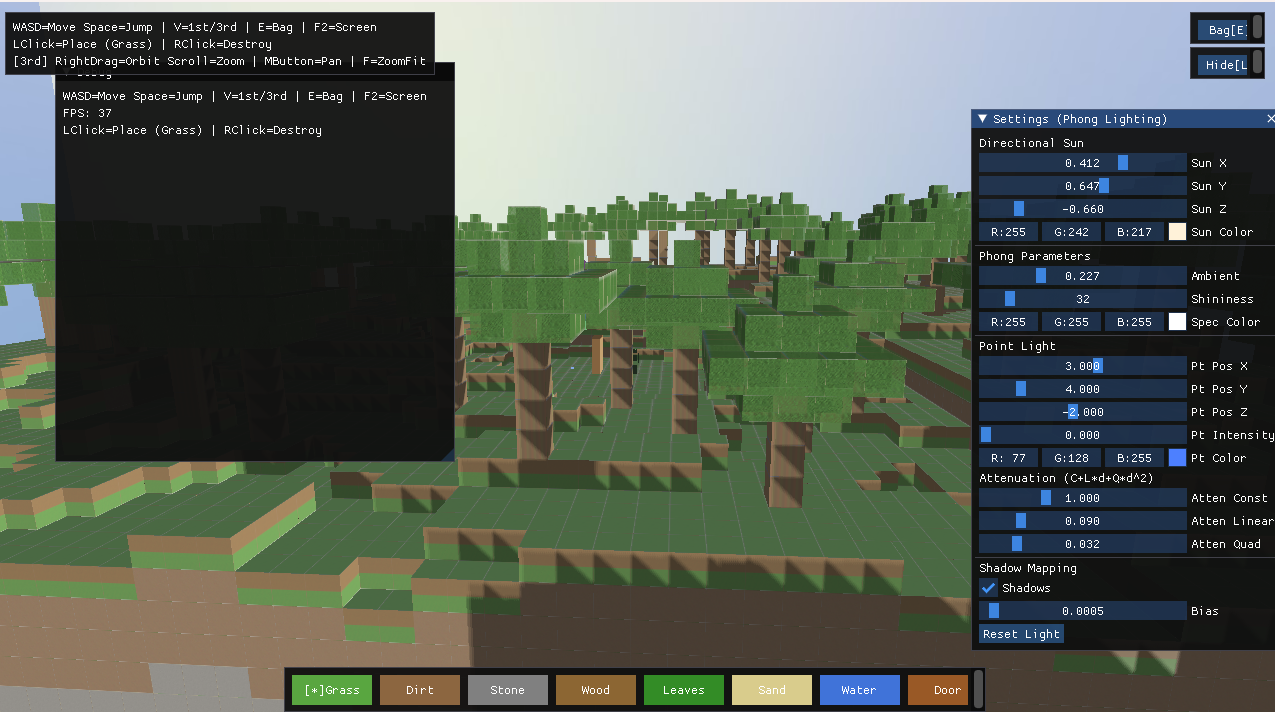
\includegraphics[width=0.75\textwidth]{figures/shadow.png}
    \caption{PCF 软阴影效果展示}
    \label{fig:shadow}
\end{figure}


\subsection{完整三维游戏}

基于引擎构建了可玩的 Minecraft/TD 混合游戏 \texttt{final\_project}：

\subsubsection{核心玩法}
\begin{itemize}[nosep]
    \item \textbf{世界生成：} 程序化噪声地形（multi-octave 噪声），32×32 区块，包含树木自动放置
    \item \textbf{体素编辑：} 右键放置方块，左键破坏（掉落物品可拾取）
    \item \textbf{塔防机制：}
          \begin{itemize}
              \item 放置箭塔防御从四面八方涌来的敌人
              \item 敌人（灰骑士模型）沿地形寻路向玩家移动
              \item 波次管理系统（\texttt{WaveManager}），难度递增
              \item HUD 显示波次、生命值、得分
          \end{itemize}
    \item \textbf{第一/第三人称切换：} 按 \texttt{F} 键无缝切换
    \item \textbf{背包系统：} 按 \texttt{E} 键打开背包，九宫格热键栏
    \item \textbf{场景装饰：} 悬浮地球仪 + 轨道旋转的基本图元展示
\end{itemize}

\subsubsection{视觉特性}
\begin{itemize}[nosep]
    \item 程序化生成的天空盒（雪山 + 湖景），6 面无缝拼接
    \item 实时阴影覆盖所有方块和角色
    \item 半透明水面渲染（alpha blending）
    \item 昼夜循环效果（通过调整太阳方向实现）
    \item 角色骨骼动画（idle/walk/jump 平滑过渡）
\end{itemize}

\begin{figure}[H]
    \centering
    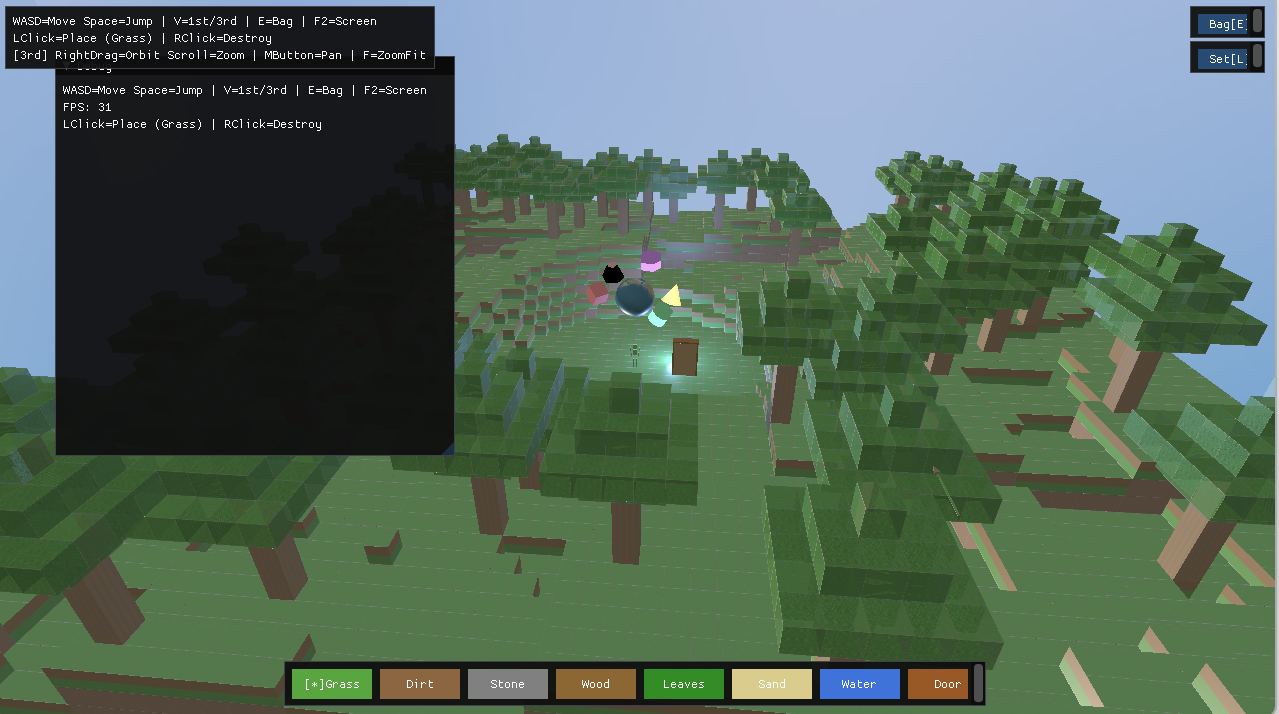
\includegraphics[width=0.85\textwidth]{figures/total.png}
    \caption{游戏总览截图}
    \label{fig:total}
\end{figure}


\subsection{对象表达能力（门、窗、墙）}

实现了具有实际功能差异的建筑对象系统：

\begin{itemize}[nosep]
    \item \textbf{门：}
          \begin{itemize}
              \item 由门框（左右柱 + 上梁 + 下梁）和门扇组成
              \item 关闭时：实心碰撞体积，不可通行
              \item 打开时：门扇旋转 90°，碰撞 AABB 实时更新；左右柱和顶梁保持碰撞
              \item 按键交互开关（\texttt{O} 键）
              \item 木质配色（深棕色门框 + 浅棕色门扇）
          \end{itemize}
    \item \textbf{窗：}
          \begin{itemize}
              \item 半透明玻璃方块（BT\_WATER 类型复用，带 alpha）
              \item 可被破坏（掉落物品）
              \item 无碰撞体积（玩家可穿过）
          \end{itemize}
    \item \textbf{墙：}
          \begin{itemize}
              \item 石头/泥土方块堆叠，始终不可通行
              \item 标准 AABB 碰撞检测
          \end{itemize}
\end{itemize}

这三种建筑对象的行为差异明确：\textbf{门}可交互开关、\textbf{窗}可穿过可破坏、\textbf{墙}始终阻塞。符合“关闭的门不可通行，可以按键打开，打开后可通行；窗可打碎、翻越；墙始终不可通行”的要求。

% ============================================================
\section{核心算法详解}
% ============================================================

\subsection{地形生成算法}

采用多层叠加的 2D 噪声函数（伪随机哈希 + 平滑插值）：

\begin{lstlisting}[language=C++]
float MinecraftGame::getTerrainHeight(float wx, float wz) const {
    float h = 0;
    h += noise2D(wx * 0.02f, wz * 0.02f) * 12.0f;  // 大尺度起伏
    h += noise2D(wx * 0.05f, wz * 0.05f) * 5.0f;   // 中等尺度
    h += noise2D(wx * 0.12f, wz * 0.12f) * 2.0f;   // 细节
    return h;
}
\end{lstlisting}

根据高度值分层放置方块：低于高度 → 石头，等于高度 $-1$ → 泥土，等于高度 → 草方块。低于水位线 → 沙地/水。

\subsection{碰撞检测算法}

核心采用分离轴定理（SAT）的简化版——AABB vs AABB 六轴检测：

\[
\text{overlap}(A,B) \iff 
\begin{cases}
A.\text{min}_x < B.\text{max}_x \;\land\; A.\text{max}_x > B.\text{min}_x \\
A.\text{min}_y < B.\text{max}_y \;\land\; A.\text{max}_y > B.\text{min}_y \\
A.\text{min}_z < B.\text{max}_z \;\land\; A.\text{max}_z > B.\text{min}_z
\end{cases}
\]

滑动碰撞分三步（Y → X → Z 顺序），每一步独立检测碰撞并允许平行于墙面的滑动，实现自然的贴墙行走效果。

\subsection{门扇旋转AABB碰撞}

门扇绕合页轴旋转角度 $\theta$，其 AABB 半轴为：
\begin{align*}
h_x &= |\cos\theta| \cdot \frac{W}{2} + |\sin\theta| \cdot \frac{T}{2} \\
h_z &= |\sin\theta| \cdot \frac{W}{2} + |\cos\theta| \cdot \frac{T}{2}
\end{align*}
其中 $W$ 为门扇宽度（1.76），$T$ 为厚度（0.21）。\texttt{resolvePlayerMovement()} 中用 $\cos\theta$ 和 $\sin\theta$ 计算真实 AABB，沿最短重叠轴推出玩家，保证任意旋转角度下碰撞均精确有效。

% ============================================================
\section{运行与编译}
% ============================================================

\subsection{编译方法}
\begin{lstlisting}[language=bash]
cd final
mkdir build && cd build
cmake .. -G "Visual Studio 17 2022"
cmake --build . --config Release
\end{lstlisting}

编译产物位于 \texttt{build/bin/Release/}：
\begin{itemize}[nosep]
    \item \texttt{final\_project.exe} —— 主游戏程序
    \item \texttt{01\_primitives.exe} ～ \texttt{09\_skeletal.exe} —— 各模块演示程序
\end{itemize}

\subsection{操作说明}

\begin{itemize}[nosep]
    \item \textbf{WASD：} 移动 \quad \textbf{Space：} 跳跃
    \item \textbf{鼠标左键：} 破坏方块 \quad \textbf{鼠标右键：} 放置方块
    \item \textbf{F：} 切换第一/第三人称 \quad \textbf{E：} 打开背包
    \item \textbf{O：} 开关最近的门 \quad \textbf{P：} 截图
    \item \textbf{1–9：} 快捷栏选择方块类型
    \item \textbf{滚轮：} 第三人称缩放 \quad \textbf{右键拖拽：} 旋转视角
    \item \textbf{Esc：} 释放鼠标 \quad \textbf{Settings 面板：} 调整光源参数
\end{itemize}

% ============================================================
\section{总结与展望}
% ============================================================

本项目实现了一个功能完整的三维图形引擎，覆盖了课程要求的全部基本功能（体素建模、OBJ 导入导出、材质纹理、几何变换、Phong 光照、场景漫游、动画截图）和多项扩展功能（NURBS 曲面、AABB 碰撞检测、PCF 阴影映射、完整游戏、门/窗/墙对象系统）。

引擎采用模块化设计，各子系统（渲染、碰撞、动画、游戏逻辑）解耦清晰，便于扩展和维护。通过合理的算法选择（如 instanced rendering 优化方块绘制、PCF 软阴影提升画质、旋转 AABB 处理可动碰撞体）在功能和性能之间取得了良好平衡。

未来可扩展方向：全局光照（Voxel GI）、物理模拟（Bullet 集成）、网络多人联机、更丰富的生物群系等。

\end{document}
